\documentclass[11pt]{article}
\title{CSE 576 Project 3: Generative Discriminative Image Classifier.}
\author{Brendan Miller}
\usepackage{multirow,amsmath}
\usepackage{graphicx}
\usepackage{fancyvrb}
\usepackage{color}
\usepackage{amsfonts}
%\usepackage{hyperref}
\usepackage{longtable}
\begin{document}

\maketitle
\section{Introduction}

This project recognizes images that contain certain classes of
objects. To do this I use the generative/descriminative framework
discussed in Yi Li\cite{gendesc}.

Whereas Li's paper used features extracted from clustered abstract
regions such as color and texture, this project also uses descriptors
extracted from keypoints. Specifically, the keypoints and descriptors
generated by SIFT.

Motivation behind the project

Objective of the project

\section{Related work}

This project is primarily based on \emph{A Generative/Discriminative
  Learning Algorithm for Image Classification} by Yi
Li\cite{gendesc}. Li's generative/discriminative classifier framework
works in two stages.

First, features are extracted from a training set of positive
examples. From this set of features, the expectation maximization
algorithm is used to create a gaussian mixture model of the
distribution of the features.

For an object $o$ and a feature type $a$ the probability of a
particular feature vector $X^a$ appearing can be calculated from the
gaussian mixture model as
\begin{equation*}
  P(X^a|o) = \sum_{m=1}^{M^a} w^a_m N(X^a; \mu^a_m, \Sigma^a_m)
\end{equation*}
where $M^a$ is the number of clusters in the mixture model for feature
$a$. For the $m$th gaussian of feature $a$ $w^a_m$ is the weight,
$\mu^a_m$ is the mean, and $\Sigma^a_m$ is the covariance matrix.

In the discriminative step, both positive and negative examples are
used to train a classifier, in this case a pretty standard 3 layer
neural network.

For the $i$th image the joint probabilities of the $r$th feature
in the image and the $m$th component gaussian of feature type $a$ is
calculated like so:
\begin{equation*}
  P(X^a_{i,r},m^a) = w^a_m N(X^a_{i,r}, \mu^a_m, \Sigma^a_m)
\end{equation*}
to determine how well an image $I_i$ matched a component gaussian $m_a$, I just
use the maximum for all features in the image, given the reasoning
that having some features that do not match, should reduce the score
of the overall match:
\begin{equation*}
P(I_i, m^a) = max(\{P(X^a_{i,r}, m^a)|r \in \mbox{features of type $a$
  in the $i$th image\}})
\end{equation*}

Then to train the neural network, for each image a vector is created
that corresponds to an input to the training stage of the neural
network. For image $I_i$ and for all guassian components $m^a$ for all
feature types $a$ the vector contains $P(I_i, m^a)$. The neural
network is trained to return 1 for vectors from positive example
images, and 0 for negative examples.

In practice, given a vector of maximum joint probabilities, the neural
network will return a value roughly between 0 and 1 that corresponds
to the confidence that object $o$ is present. For this reason, a
threshold over the output of the neural network can be varied to trade
off the likely number of false positives and false negatives
returned. In my implementation I use a threshold of 0.5.

\section{Your method}

My implementation keeps the underlying framework of Li's paper, but in
additional to using reagional features, also uses descriptors from
keypoints.

In my implementation for each image I extracted SIFT\cite{sift}
descriptors using the OpenCV library and fed these into the generative
descriminative framework discussed in the last section.

I found that using a fairly large number of component guassians in the
SIFT mixture model helped greatly with classification accuracy. I believe this
is because a given object class can have many distinctive parts, and a
component gaussian is needed to represent each.

Using a SIFT guassian mixture model with 50 components, I could
achieve classification accuracy upwards of 80\%  with most objects,
and much higher with some.

The number of gaussian components can continue to be increased to
increase accuracy. I capped it at 50 for most of my testing mainly
because the computational overhead became significant with higher
numbers of gaussians.

In addition to SIFT descriptors, I also ran kmeans on each image to
extract color clusters, the mean color of which I fed into the
generative/descriminative framework.

Color is mainly useful for classifying objects that have a distintive
color, such as faces which contain the human skin color. They were
less useful for classifying cars, planes, and motorcycles, which
all can be painted a variety of colors.

\section{Experiments and results}

Describe the datasets that you used

Evaluation criteria

Performance evaluation:

Analysis of the performance

Use images, tables and graphs to help describe your results

Classification accuracy using both color and SIFT features:

\begin{tabular}{| l | l | l | l |}
  \hline
  Image Type & Accuracy     & False Positives    & False Negatives \\
  Cars      & 0.94  & 0.035 & 0.025 \\
  Planes    & 0.78  & 0.11  & 0.11  \\
  Faces     & 0.9   & 0.055 & 0.045 \\
  Bikes     & 0.805 & 0.08  & 0.115 \\
  \hline
\end{tabular}

This is an example of a correctly classified plane.

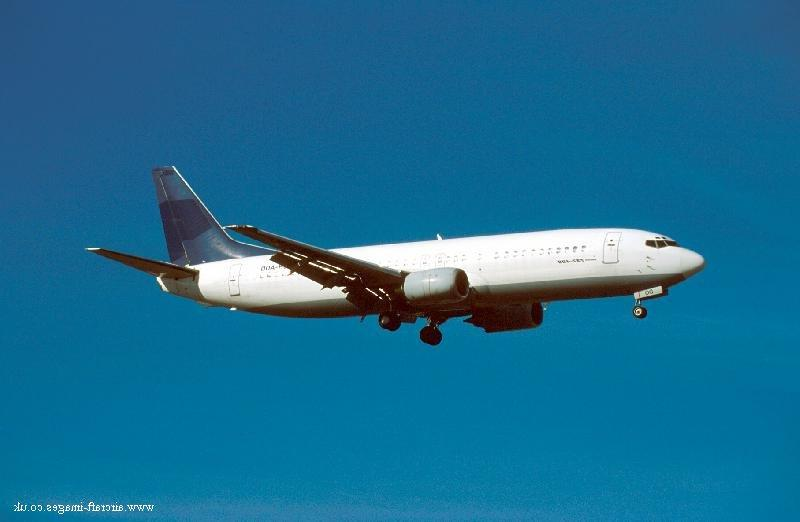
\includegraphics[width=100mm]{images/plane_true_positive.png}

False positives:
It's a little tricky to interpret why this example was classified as a
plane, but my guess is that the white color of the car, which is more
common on commercial aircraft then in automobiles, partially had to do
with it.

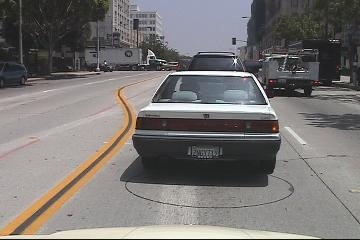
\includegraphics[width=100mm]{images/plane_false_positive.png}

False negatives:
Here's an example of a false negative during face classification. This
image lacks the distinctive color of skin, and is also hand drawn so
keypoint descriptors may not be quite the same as with real faces.

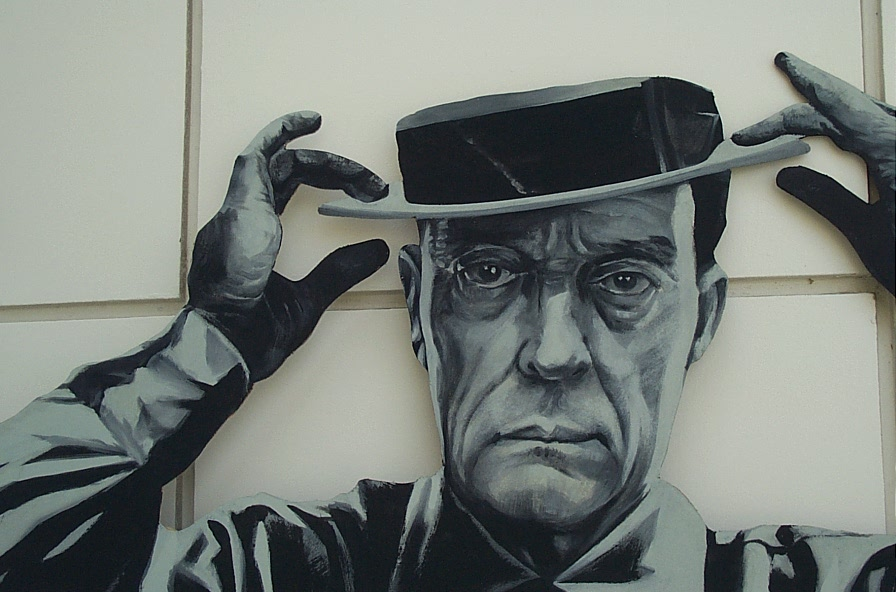
\includegraphics[width=100mm]{images/face_false_negative.png}


\section{5. Future work}

Idea: Keep track of regions as they move through framework so you can
determine what areas of image were most responsible for positive
classification.

Will need to use something other than a neural network for this, since
a neural network is a little too hard to interpret, and figure out
which inputs were most responsible for result.

The idea is to avoid the need to train a separate classifier that has
carefully cropped training data (e.g. the Viola Jones algorithm), but
rather to be able to use the messy data present in the wild for
training.

TODO:Possible future extensions to the project.

The original descrimitive generative paper also included texture and
structural features, so an obvious extension would be to include those
features as well.

Beyond that, finding higher performance means of extracting features
similar to the existing ones would mak it practical to include more
features in the classifier.

In particular, since running k means on input images to perform
classification is somewhat time consuming for real time applications,
more efficient means of extracting color features might be tried. For
instance, a color histogram might be formed, and the peak bins of the
histogram used as features.

Even if the more efficient features are less predictive individually,
since they allow time for additional features to be computed, the
classifier overall could have better performance.

An alternative approach might be to extract different feature classes
simultaniously in different threads.


\section{Summary and conclusion}

\begin{thebibliography}{9}

\bibitem{gendesc}
  Y. Li, L. G. Shaprio, and J. Bilmes
  \emph{A Generative/Discriminative Learning Algorithm for Image Classification}.
  Department of Computer Science and Engineering,
  Department of Electrical Engineering,
  University of Washington

\bibitem{sift}
  David G. Lowe
  \emph{Distinctive Image Features from Scale-Invariant Keypoints}
  Computer Science Department
  University of British Columbia
  Vancouver, B.C., Canada
  January 5, 2004

\end{thebibliography}

\end{document}
